\subsection{Discriminative relational tasks}\label{ssec:experiments_discriminative}

\subsubsection{Order relations: modeling asymmetric relations}
A recent closely related work is~\citep{kerg2022neural}, which identifies and argues for certain inductive biases in relational models. They propose a model called CoRelNet which is, in some sense, the simplest possible model which satisfies those inductive biases. They show that this model is capable of outperforming several previous explicitly relation architectures. One inductive bias which they argue for is to model relations between objects as \textit{symmetric} inner products between object representations. In this section, we aim to add to the discussion on inductive biases for relational learning by arguing that a general relational architecture needs to be able to model asymmetric relations as well.

The CoRelNet architecture is as follows: given a sequence of objects $(x_1, \ldots, x_m)$, embed them by some embedder $\phi$, then compute the similarity matrix $R = \text{Softmax}(A), A = {\left[\langle\phi(x_i), \phi(x_j)\rangle\right]}_{ij}$. In this form, CoRelNet models relations as necessarily symmetric. It can be modified to support asymmetric relations via the natural modification $A = {\left[\langle W_1 \phi(x_i), W_2 \phi(x_j)\rangle\right]}_{ij}$, where $W_1, W_2$ are trainable matrices. In~\citep{kerg2022neural} the authors argue that symmetry is an important inductive bias. The following simple experiment demonstrates that, while symmetry may be a useful inductive bias on relational tasks where the underlying relation is symmetric, the ability to model asymmetric relations is necessary for more general tasks.

% Another limitation is that it can only model single-dimensional relations---for each pair of objects $(i,j)$, their modeled relation is a single-dimensional scalar $R_{ij}$. The Abstractor is able to model a significantly larger class of relations. In particular, it is able to model asymmetric and multi-dimensional relations through the $\text{MultiHeadRelation}$ operation. This is demonstrated by the following simple experiment.

\textbf{Experimental details:} We generate $N = 32$ ``random objects'' represented by iid Gaussian vectors, $o_i \overset{iid}{\sim} \mathcal{N}(0,
I_d) \in \mathbb{R}^d$, and associate an order relation to them $o_1 \prec o_2 \prec \cdots \prec o_N$. Note that $\prec$ is \textit{not symmetric}. Of the $N^2 = 1024$ possible pairs $(o_i, o_j)$, 15\% are held out as a validation set (for early stopping) and 35\% as a test set. We evaluate learning curves by training on the remaining 50\% and computing accuracy on the test set (10 trials for each training set size). Note that under this set up, we are evaluating the models on pairs they have never seen. Thus, the models will need to generalize based on the transitivity of the $\prec$ relation.

We compare three models: an Abstractor, standard (symmetric) CoRelNet, and asymmetric CoRelNet. We observe that standard symmetric CoRelNet is completely unable to learn the task, whereas the Abstractor and asymmetric CoRelNet learn the transitive $\prec$ relation~(\Cref{fig:exp_order_relation}).~\citep{kerg2022neural} finds symmetry to be an important inductive bias for the relational tasks they consider (which are based on a simple same/different underlying relation), whereas we find that the ability to model asymmetric relations is necessary for more general tasks. This can be explained in terms of the relational bottleneck. In a relational task, there exists a sufficient statistic which is relational. The relational bottleneck restricts the space of learnable representations to be the space of relational features, thus making the search for a good representation easier and more sample efficient. In a relational task in which there exists a sufficient statistic involving a symmetric relation (as is the case with same/different tasks), we can further restrict the search space to be over symmetric relational representations, which should make learning a good representation even more sample efficient. Since the experiments \citep{kerg2022neural} considers are indeed symmetric, symmetry was a useful inductive bias. However, some relations are more complex and may be asymmetric---an example is order relations. Symmetric inner products don't have the representational capacity to model such relations. But asymmetric inner products with different learned left and right encoders can model such relations.

\subsubsection{SET: modeling multi-dimensional relations}

The $\prec$ relation is a one-dimensional relation. Similarly, the underlying relations in the experiments considered in~\citep{kerg2022neural} are also one-dimensional (same/different). In the next experiment, we explore a discriminative relational tasks which relies on a multi-dimensional relation. The task we consider is SET. 

\begin{wrapfigure}{R}{0.25\textwidth}
	\vskip-5pt
	\begin{tabular}{c}
		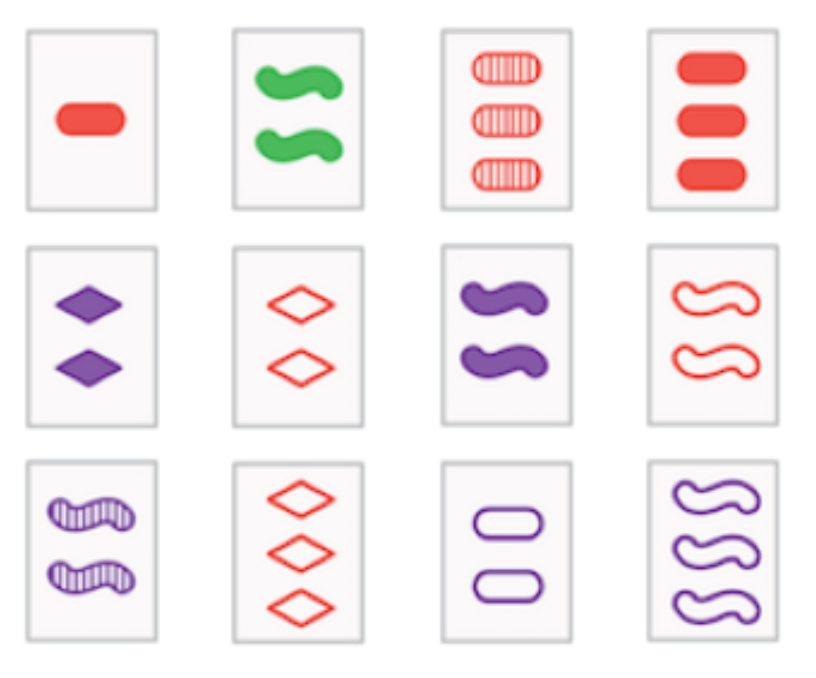
\includegraphics[width=.25\textwidth]{figures/set_example}\\[-5pt]
	\end{tabular}
	\caption{\footnotesize The SET game}
\end{wrapfigure}
SET is a relatively straightforward but challenging cognitive task that engages reasoning faculties in a deliberative, attentionally directed manner, requiring several levels of abstraction over sensory embeddings. Players are
presented with 12 cards, each of which contains figures that vary along four dimensions (color, number, pattern, and
shape) and they must find subsets of three cards which obey a deceptively simple rule: along each dimension, all cards in a SET must either have the same or unique values.
For example, in the figure to the right, the cards with two solid blue/purple diamonds, two striped blue squiggles, and two open blue oblongs form a SET: same color, same number, different patterns, different shapes.

\textbf{Experimental details:} The task is, given a triplet of card images, to determine whether they form a set or not. A CNN classifier is trained on the card images to predict the four attributes. An intermediate layer is used as an embedder for all relational models. We compare an Abstractor model to CorelNet. The shared architecture is CNN embedder $\to$ Dense $\to$ \{Abstractor or CorelNet\} $\to$ Flatten $\to$ Dense $\to$ Prediction. The CNN is trained to predict the four attributes of
each card and then an embedding of dimension $d=32$ of each card is obtained from an intermediate layer. The Abstractor has hyperparamaters: 2 layers, 4-dimensional symmetric relations, linear relation activation. We tested against the standard version of CorelNet, but found that it did not learn anything. We iterated over the hyperparamters and architecture to improve its performance. We found that removing the softmax activation in CoRelNet improved performance a bit. We report learning curves in~\Cref{fig:exp_set_classification} (10 trials per training set size). We find that the Abstractor model significantly out-performs both variants of CoRelNet. We attribute this to its ability to model multi-dimensional relations. In this task, there exists four different relations (one for each attribute) which are needed to determine whether a triple of cards forms a set. CoRelNet would need to squeeze all of this information into a single-dimensional scaler whereas the Abstractor can model each relation separately. We hypothesize that the ability to model relations as multi-dimensional is also the reason that the Abstractor can learn the order relation better than asymmetric CoRelNet---even though the underlying relation is one-dimensional, having a multi-dimensional representation enables greater robustness and multiple avenues towards a good solution during optimization.


\begin{figure}[t]
    % \vskip-.2in
    \begin{subfigure}[t]{0.30\textwidth}
        %\centering
        %\hskip-.35in
        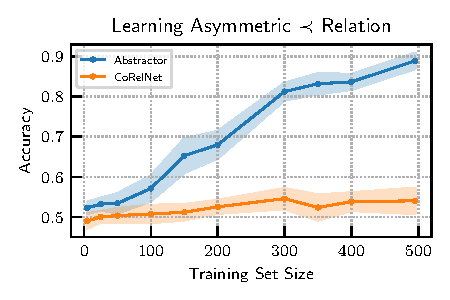
\includegraphics[width=1.1\textwidth]{figures/experiments/pairwise_order_learning_curves.pdf}
        % \vskip-5pt
        \caption{The $\prec$ relation can be learned with asymmetric but not symmetric inner products.}\label{fig:exp_order_relation}
    \end{subfigure} 
    \hskip10pt
    % \captionsetup[subfigure]{oneside,margin={-.3in,0in}}
    \begin{subfigure}[t]{0.30\textwidth}
        %\centering
        % \vskip10pt
        % \hskip-.6in
        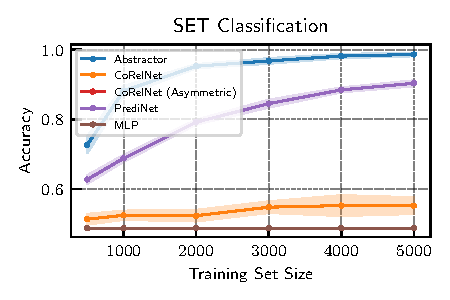
\includegraphics[width=1.1\textwidth]{figures/experiments/set_classification.pdf}
        % \vskip-5pt
        \caption{The Abstractor's ability to model multi-dimensional relations enables it to solve SET.}\label{fig:exp_set_classification}
    \end{subfigure}
    \caption{Experiments on discriminative relational tasks and comparison to CoRelNet.}
\end{figure}
